\let\negmedspace\undefined
\let\negthickspace\undefined
\documentclass[journal]{IEEEtran}
\usepackage[a5paper, margin=10mm, onecolumn]{geometry}
%\usepackage{lmodern} % Ensure lmodern is loaded for pdflatex
\usepackage{tfrupee} % Include tfrupee package

\setlength{\headheight}{1cm} % Set the height of the header box
\setlength{\headsep}{0mm}  % Set the distance between the header box and the top of the text

\usepackage{gvv}
\usepackage{cite}
\usepackage{amsmath,amssymb,amsfonts,amsthm}
\usepackage{algorithmic}
\usepackage{graphicx}
\usepackage{textcomp}
\usepackage{xcolor}
\usepackage{txfonts}
\usepackage{listings}
\usepackage{enumitem}
\usepackage{mathtools}
\usepackage{gensymb}
\usepackage{comment}
\usepackage[breaklinks=true]{hyperref}
\usepackage{tkz-euclide}
\def\inputGnumericTable{}                                 
\usepackage[latin1]{inputenc}                                
\usepackage{color}                                            
\usepackage{array}                                            
\usepackage{longtable}                                       
\usepackage{calc}                                             
\usepackage{multirow}                                         
\usepackage{hhline}                                           
\usepackage{ifthen}                                           
\usepackage{lscape}

% Corrected equation environment commands
\newcommand{\BEQA}{\begin{eqnarray}}
\newcommand{\EEQA}{\end{eqnarray}}
\newcommand{\define}{\stackrel{\triangle}{=}}

\begin{document}

\bibliographystyle{IEEEtran}
\vspace{3cm}

\title{3-3.2-26}
\author{AI24BTECH11006 - Bugada Roopansha}

{\let\newpage\relax\maketitle}  % Prevents the new page after title

\renewcommand{\thefigure}{\theenumi}
\renewcommand{\thetable}{\theenumi}
\setlength{\intextsep}{10pt} % Space between text and floats

\textbf{Question:}\\
Construct a right triangle when one side is 3.5 cm, the sum of the other side and the hypotenuse is 5.5 cm.

\textbf{Solution:}\\
For \( a = 3.5 \, \text{cm} \), \( \angle B = 90\degree \), and \( b + c = 5.5 \, \text{cm} \), we can find the lengths of sides \( b \) and \( c \) to complete the triangle. The plot below illustrates the right triangle constructed based on these parameters.

\begin{figure}[h!]
\centering
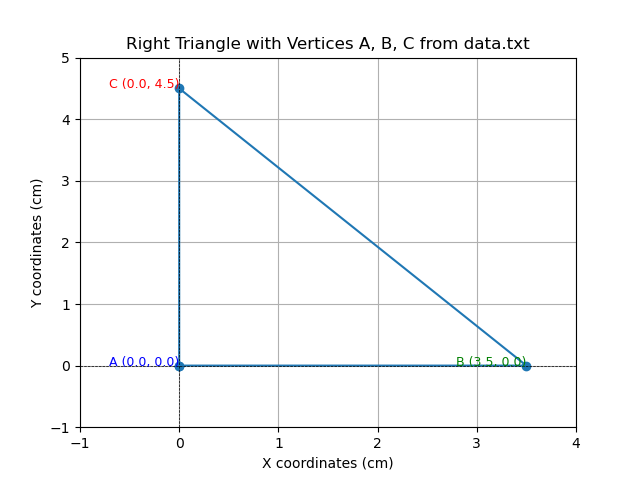
\includegraphics[width=1\textwidth]{fig.png} % Replace with your image file
\caption{Right triangle with one side of 3.5 cm and the sum of the other side and hypotenuse equal to 5.5 cm.}

\end{figure}

\end{document}

